\section{Supplementary pooling, metrics, and uncertainty}
\label{sec:supplement}
The supplementary \meanmodel{} uses the same training seeds 21/44, folds, observed-history protocol, future-state objective, and forecast classifier feature groups as \fullmodel{}, replacing spatial attention with mean pooling. Only the equal two-seed aggregate is presented, consistent with the main analysis.
\begin{table*}[t]
\centering
\small
\caption{Supplementary pooling comparison using the same two-seed aggregation as the main analysis. ForecastMean and ForecastAttention share forecast readout and future-state supervision, differing in spatial pooling.}
\label{tab:pooling}
\begin{tabular}{llrrr}
\toprule
Model & Landmark & AUROC & AP & F1 \\
\midrule
ForecastMean & T0 & 0.7322 & 0.5863 & 0.5354 \\
ForecastMean & T1 & 0.7339 & 0.5902 & 0.5355 \\
ForecastMean & T2 & 0.7322 & 0.5865 & 0.5273 \\
ForecastMean & Macro & 0.7328 & 0.5877 & 0.5327 \\
ForecastAttention & T0 & 0.7323 & 0.5933 & 0.5391 \\
ForecastAttention & T1 & 0.7363 & 0.5976 & 0.5524 \\
ForecastAttention & T2 & 0.7393 & 0.5998 & 0.5556 \\
ForecastAttention & Macro & 0.7360 & 0.5969 & 0.5490 \\
\bottomrule
\end{tabular}
\end{table*}

\begin{table*}[t]
\centering
\footnotesize
\setlength{\tabcolsep}{5pt}
\caption{All 14 macro metrics for the principal variants: point estimate [95\% patient-bootstrap percentile interval]. Each statistic averages fold metrics within seed, equally averages seeds 21/44, and equally averages T0--T2. Threshold-dependent metrics use 0.5. Identical patient resamples preserve pairing across models, folds, seeds, and landmarks; entries are marginal model intervals, rather than intervals for differences. Intervals condition on the fitted models and exclude retraining and retrospective selection uncertainty. Downward arrows identify metrics for which lower is better.}
\label{tab:extended_macro}
\begin{tabular}{lccc}
\toprule
Metric & NoJEPA & DirectReadout & ForecastAttention \\
\midrule
AUROC & 0.7157 [0.6432, 0.7893] & 0.7277 [0.6560, 0.8007] & 0.7360 [0.6656, 0.8063] \\
AP & 0.5773 [0.4588, 0.6935] & 0.5904 [0.4701, 0.7061] & 0.5969 [0.4841, 0.7136] \\
F1 & 0.5333 [0.4332, 0.6247] & 0.5425 [0.4421, 0.6326] & 0.5490 [0.4598, 0.6319] \\
Accuracy & 0.6743 [0.6168, 0.7307] & 0.6790 [0.6202, 0.7362] & 0.6509 [0.5985, 0.7038] \\
Sensitivity & 0.5875 [0.4780, 0.6994] & 0.5970 [0.4847, 0.7132] & 0.6673 [0.5698, 0.7639] \\
Specificity & 0.7151 [0.6460, 0.7810] & 0.7176 [0.6490, 0.7841] & 0.6431 [0.5770, 0.7076] \\
PPV & 0.4954 [0.3861, 0.6083] & 0.5011 [0.3921, 0.6167] & 0.4796 [0.3817, 0.5831] \\
NPV & 0.7888 [0.7170, 0.8592] & 0.7922 [0.7198, 0.8609] & 0.8143 [0.7456, 0.8797] \\
Balanced accuracy & 0.6513 [0.5860, 0.7171] & 0.6573 [0.5915, 0.7241] & 0.6552 [0.6003, 0.7140] \\
MCC & 0.2931 [0.1656, 0.4208] & 0.3037 [0.1773, 0.4281] & 0.3013 [0.1949, 0.4120] \\
Youden index & 0.3026 [0.1719, 0.4342] & 0.3147 [0.1830, 0.4481] & 0.3104 [0.2005, 0.4279] \\
NLL $\downarrow$ & 0.6018 [0.5403, 0.6624] & 0.5959 [0.5318, 0.6605] & 0.6102 [0.5592, 0.6611] \\
Brier score $\downarrow$ & 0.2083 [0.1825, 0.2347] & 0.2049 [0.1783, 0.2324] & 0.2118 [0.1903, 0.2334] \\
ECE $\downarrow$ & 0.1323 [0.1127, 0.1916] & 0.1280 [0.1101, 0.1868] & 0.1544 [0.1253, 0.2128] \\
\bottomrule
\end{tabular}
\end{table*}

\begin{table*}[t]
\centering
\small
\caption{Exploratory paired patient-bootstrap intervals for three-landmark mean differences (2,000 shared patient draws). Intervals condition on the fitted models and exclude retraining and seed-selection uncertainty.}
\label{tab:bootstrap}
\begin{tabular}{llr}
\toprule
Comparison & Metric & Difference [95\% interval] \\
\midrule
DirectReadout -- NoJEPA & AUROC & +0.0120 [+0.0011, +0.0242] \\
DirectReadout -- NoJEPA & AP & +0.0131 [-0.0013, +0.0261] \\
DirectReadout -- NoJEPA & F1 & +0.0092 [-0.0066, +0.0250] \\
ForecastAttention -- NoJEPA & AUROC & +0.0203 [+0.0042, +0.0381] \\
ForecastAttention -- NoJEPA & AP & +0.0196 [-0.0064, +0.0473] \\
ForecastAttention -- NoJEPA & F1 & +0.0157 [-0.0093, +0.0409] \\
ForecastAttention -- DirectReadout & AUROC & +0.0083 [-0.0041, +0.0215] \\
ForecastAttention -- DirectReadout & AP & +0.0065 [-0.0150, +0.0311] \\
ForecastAttention -- DirectReadout & F1 & +0.0065 [-0.0178, +0.0326] \\
\bottomrule
\end{tabular}
\end{table*}

\begin{table*}[t]
\centering
\small
\caption{Three-landmark mean operating-point sensitivity analysis, equally averaged over seeds 21 and 44 after within-seed five-fold aggregation. The alternative threshold maximizes Youden index separately on each fold and landmark validation set; the highest threshold breaks ties. No holdout predictions select thresholds. Probability-based AUROC and AP are unchanged by this operation.}
\label{tab:extended_threshold}
\begin{tabular}{llrrrr}
\toprule
Model & Policy & F1 & Sens. & Spec. & MCC \\
\midrule
NoJEPA & 0.5 & 0.533 & 0.588 & 0.715 & 0.293 \\
NoJEPA & Validation Youden & 0.535 & 0.614 & 0.684 & 0.285 \\
\midrule
DirectReadout & 0.5 & 0.542 & 0.597 & 0.718 & 0.304 \\
DirectReadout & Validation Youden & 0.537 & 0.601 & 0.706 & 0.298 \\
\midrule
ForecastAttention & 0.5 & 0.549 & 0.667 & 0.643 & 0.301 \\
ForecastAttention & Validation Youden & 0.542 & 0.640 & 0.661 & 0.288 \\
\bottomrule
\end{tabular}
\end{table*}


\begin{figure*}[t]
\centering
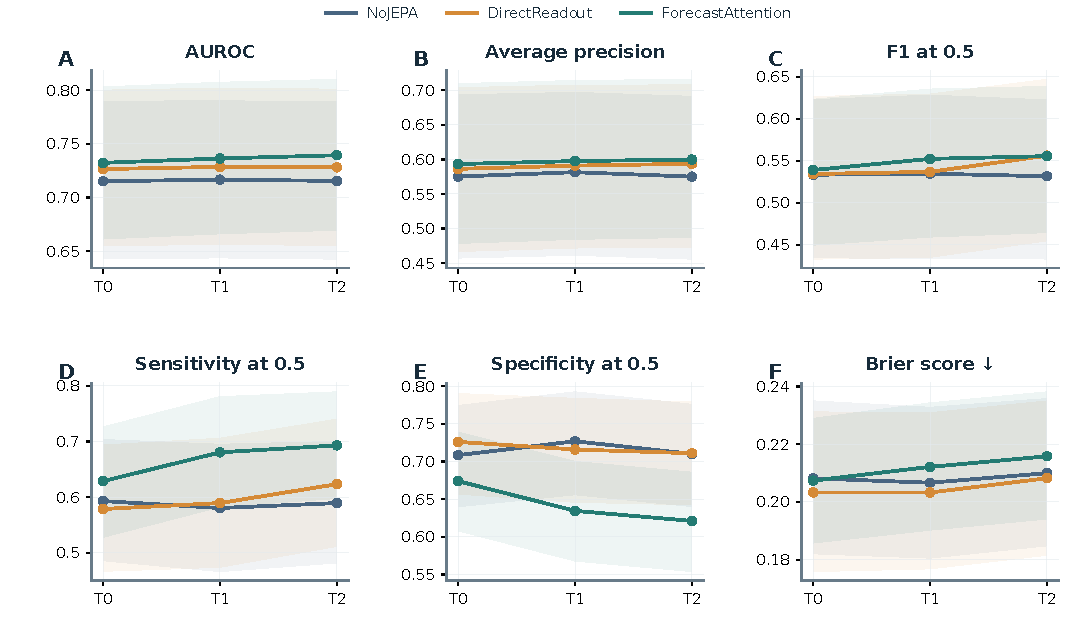
\includegraphics[width=\textwidth]{figures/landmark_performance.pdf}
\caption{Six complementary landmark summaries: AUROC, AP, F1, sensitivity, specificity, and Brier score. All points use fold-then-seed aggregation; shading is the conditional 95\% patient-bootstrap interval. The same 175 patients appear at every landmark. A trend in ranking can coexist with a different trend in calibration or error types.}
\label{fig:longitudinal}
\end{figure*}

\begin{figure*}[t]
\centering
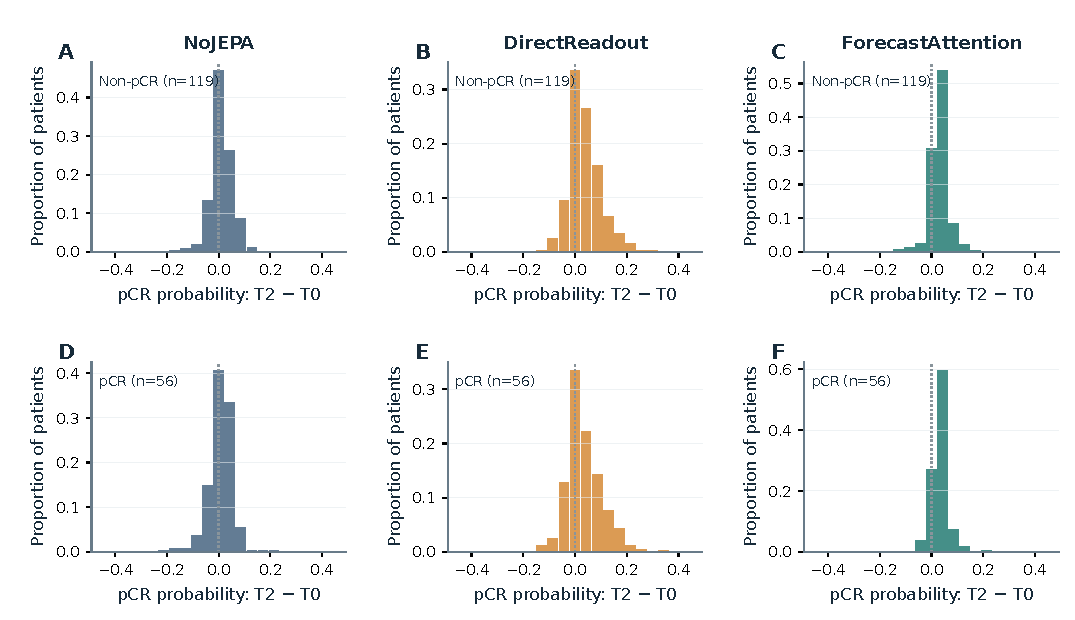
\includegraphics[width=\textwidth]{figures/outcome_score_changes.pdf}
\caption{Outcome-conditioned changes in predicted pCR probability from T0 to T2. Panels separate models and outcome classes. Histograms are computed within each fitted model and then averaged over folds and seeds; they are not histograms of probability-ensemble predictions. Changes describe model scores and do not establish an individual treatment effect.}
\label{fig:scorechanges}
\end{figure*}

\section{Supplementary subgroup and training-probe summaries}
\begin{table*}[t]
\centering
\small
\caption{Exploratory subgroup discrimination for the equal-weight seeds 21/44 mean. AUROC is averaged over five folds within each seed, then seeds 21/44 equally, and T0--T2; intervals are paired patient-bootstrap intervals for ForecastAttention minus NoJEPA, conditional on the fixed models. Age 50 is an exploratory reporting cutpoint. Namespace groups are parts of one clinical release, not external cohorts.}
\label{tab:subgroups}
\begin{tabular}{lrrr}
\toprule
Subgroup ($n$/pCR+) & NoJEPA & Full & $\Delta$ AUROC [95\% interval] \\
\midrule
HR+/HER2- (68/11) & 0.659 & 0.711 & +0.052 [+0.009, +0.099] \\
HR+/HER2+ (31/12) & 0.636 & 0.621 & -0.015 [-0.078, +0.047] \\
HR-/HER2+ (14/7) & 0.812 & 0.816 & +0.004 [-0.113, +0.099] \\
HR-/HER2- (62/26) & 0.632 & 0.654 & +0.022 [-0.009, +0.054] \\
Age $<$50 (90/29) & 0.658 & 0.685 & +0.027 [+0.006, +0.049] \\
Age $\geq$50 (85/27) & 0.774 & 0.793 & +0.019 [-0.007, +0.049] \\
ISPY2 namespace (125/39) & 0.674 & 0.692 & +0.018 [-0.003, +0.042] \\
ACRIN-6698 namespace (50/17) & 0.826 & 0.851 & +0.025 [-0.001, +0.057] \\
\bottomrule
\end{tabular}
\end{table*}

\begin{table*}[t]
\centering
\small
\caption{Archived epoch 20 fixed-training-probe diagnostics, averaged within each seed over five folds and then equally over seeds 21/44. Skill is $1-\mathrm{L1}_{forecast}/\mathrm{L1}_{copy}$ within the corresponding EMA coordinates; positive is better than holding the landmark state constant. These are training-probe summaries, not best-checkpoint holdout forecast evaluations. NoJEPA has no trained-world diagnostic.}
\label{tab:worldprobe}
\begin{tabular}{lrrr}
\toprule
Model & Horizon 1 skill & Horizon 2 skill & Horizon 3 skill \\
\midrule
NoJEPA & -- & -- & -- \\
DirectReadout & +0.023 & +0.037 & +0.158 \\
ForecastAttention & -0.029 & -0.027 & +0.017 \\
\bottomrule
\end{tabular}
\end{table*}


\section{Reproducibility and reporting items to complete}
The source package includes aggregate CSV files, source-report hashes, reproducible metric and figure scripts, the bootstrap procedure, and the official article class. It contains no patient identifiers, patient-level prediction rows, original MRI volumes, or model checkpoints. The method figure includes only rendered, anonymous development-image slices. Training seeds 21 and 44 are averaged equally after within-seed fold aggregation. Seed-specific aggregates are retained for numerical audit but are not separate manuscript results.

\todo{Before submission, complete author and ethics statements; verify the precise pCR pathology definition; document codec and segmentation patient-level pretraining provenance; add matched external baselines and a prospectively locked seed-selection policy; audit external-cohort independence; and confirm the journal's current submission and anonymization requirements.}
